\documentclass[12pt,letterpaper]{article}

% -------------------- Paquetes --------------------
\usepackage[utf8]{inputenc}
\usepackage[T1]{fontenc}
\usepackage[spanish]{babel}
\usepackage{geometry}
\geometry{margin=2.5cm}
\usepackage{setspace}
\onehalfspacing
\usepackage{graphicx}
\usepackage{float}
\usepackage{caption}
\usepackage{subcaption}
\usepackage{siunitx}
\sisetup{detect-all, round-mode=places, round-precision=3}
\usepackage{hyperref}
\usepackage{xcolor}
\usepackage{fancyhdr}
\usepackage{tikz}
\usepackage{eso-pic}
\usepackage{booktabs}
\usepackage{tabularx}
\usepackage{array}
\usepackage{amsmath}
\usepackage{amssymb}
\usepackage{listings}

\hypersetup{colorlinks=true, linkcolor=blue, urlcolor=blue}

% -------------------- Listings (VHDL) --------------------
\lstdefinelanguage{VHDL}{
  morekeywords=[1]{library,use,all,entity,is,port,in,out,end,architecture,of,begin,process,signal,if,then,elsif,rising_edge,else,when,others,generic,map,case,variable,for,loop,nor,xor,and,or,not,downto,to,wait,constant,type,array,component},
  morekeywords=[2]{std_logic,std_logic_vector,signed,unsigned,integer,std_logic_1164,numeric_std,time},
  sensitive=true,
  morecomment=[l]{--},
  morestring=[b]"
}
\lstset{
  language=VHDL,
  basicstyle=\ttfamily\small,
  frame=single,
  numbers=left,
  numberstyle=\tiny,
  breaklines=true,
  tabsize=2,
  captionpos=b
}

% -------------------- Encabezado / Pie --------------------
\pagestyle{fancy}
\fancyhf{}
\lhead{\textbf{P26-LIS2022-1}}
\rhead{\textbf{Práctica 4:} Máquinas de Estado Finito}
\renewcommand{\headrulewidth}{0.4pt}

\fancyfoot[C]{\small
\begin{tabular}{c}
186028; \href{mailto:robbie.curiosodr@udlap.mx}{robbie.curiosodr@udlap.mx}
\end{tabular}
}
\fancyfoot[R]{\small \thepage}

% -------------------- Marca de agua UDLAP --------------------
\AddToShipoutPictureBG{%
  \begin{tikzpicture}[remember picture,overlay]
    \node[opacity=0.08, rotate=12, anchor=south east] at ([xshift=1.8cm,yshift=-1.6cm]current page.south east)
    {
\includegraphics[width=0.75\paperwidth]{udlap_logo.png}};
  \end{tikzpicture}
}

\setlength{\parskip}{6pt}
\setlength{\parindent}{0pt}

\newcolumntype{L}[1]{>{\raggedright\arraybackslash}p{#1}}
\newcolumntype{C}[1]{>{\centering\arraybackslash}p{#1}}

\graphicspath{{../imagenes/}}

\begin{document}

% ========================= PORTADA =========================
\begin{titlepage}
\thispagestyle{empty}
\begin{center}
\vspace*{0.8cm}

{\Large \textsc{Universidad de las Américas Puebla}}\par
{\small Departamento de Computación, Electrónica y Mecatrónica}\par

\vspace{1.2cm}

{\Huge \textbf{Reporte de práctica}}\par
\vspace{0.15cm}
{\Large \textbf{Práctica 4: Máquinas de Estado Finito (Control Unit)}}\par

\vspace{1.0cm}

\begin{minipage}{0.92\textwidth}
\rule{\textwidth}{0.8pt}\par
\vspace{0.35cm}

\begin{tabular}{@{}L{0.30\textwidth}L{0.62\textwidth}@{}}
\textbf{Materia} & P26-LIS2022-1\\
& Arquitecturas Computacionales\\
\textbf{Profesor} & Dr. Omar Guillén Fernández\\
\textbf{Sección} & 2\\
\textbf{Periodo} & Primavera 2026\\
\end{tabular}

\vspace{0.35cm}
\rule{\textwidth}{0.8pt}
\end{minipage}

\vfill

\begin{minipage}{0.92\textwidth}
\textbf{Integrante}\par
\vspace{0.25cm}
Robbie Nicolás Curioso de Salazar \hfill 186028 \hfill \href{mailto:robbie.curiosodr@udlap.mx}{robbie.curiosodr@udlap.mx}\par
\end{minipage}

\vspace{0.6cm}

\end{center}
\end{titlepage}

% ========================= CONTENIDO =========================
\section{Introducción}
Las máquinas de estado finito (\textit{Finite State Machines}, FSM) son uno de los modelos más utilizados en el diseño de sistemas digitales secuenciales: permiten describir el comportamiento de un circuito en función de un conjunto reducido de estados, una señal de entrada y una salida que se calcula a partir de ellos. En arquitectura computacional, las FSM aparecen como base de las unidades de control, los detectores de secuencia, los protocolos serie y, en general, en cualquier circuito en el que la respuesta dependa de la historia previa de las entradas.

En esta práctica se diseñaron e implementaron en VHDL tres FSM con propósitos distintos. Las dos primeras son detectores de la secuencia binaria \texttt{101} sobre una entrada serial, una con arquitectura Mealy y otra con arquitectura Moore. La tercera es una máquina de seis estados que controla un sistema de semáforo de doble vía con cruce peatonal y que, en el diseño completo, se conecta a un divisor de frecuencia de \SI{50}{\mega\hertz} a \SI{1}{\hertz} mediante un módulo estructural de nivel superior.

El objetivo es comparar el comportamiento temporal de los modelos Mealy y Moore para una misma especificación funcional y, en paralelo, ejercitar el diseño jerárquico en VHDL combinando una unidad de control (la FSM del semáforo) con un divisor de frecuencia. La verificación funcional se realizó mediante simulación en \textit{Active-HDL} sobre tres bancos de pruebas independientes.

\section{Objetivos}
\begin{itemize}
  \item Diseñar una FSM tipo Mealy que detecte la secuencia binaria \texttt{101} sobre una entrada serial.
  \item Diseñar una FSM tipo Moore que detecte la misma secuencia y comparar su temporización con la versión Mealy.
  \item Implementar en VHDL un sistema de semáforo de doble vía con cruce peatonal mediante una FSM de seis estados.
  \item Construir un módulo estructural superior que conecte un divisor de frecuencia de \SI{50}{\mega\hertz} a \SI{1}{\hertz} con la FSM del semáforo.
  \item Validar mediante simulación en Active-HDL los tres diseños y contrastar los resultados con el comportamiento teórico esperado.
\end{itemize}

\section{Materiales y herramientas}
\begin{itemize}
  \item \textbf{Software:} Active-HDL Student Edition para compilación y simulación funcional.
  \item \textbf{Lenguaje:} VHDL, con uso de las bibliotecas \texttt{ieee.std\_logic\_1164} y \texttt{ieee.numeric\_std}.
  \item \textbf{Tecnología objetivo:} Zynq~7000 sobre tarjeta PYNQ~Z1, asumida como referencia de la frecuencia de reloj de \SI{50}{\mega\hertz}.
  \item \textbf{Documentación:} guía oficial de la práctica 4, apuntes del curso sobre FSM Mealy/Moore y la documentación de Active-HDL.
\end{itemize}

\section{Marco teórico}

\subsection{Máquinas de estado finito}
Una FSM es una abstracción de un circuito secuencial síncrono compuesto por una memoria de estado (un registro), una función de transición y una función de salida. En cada flanco activo del reloj, el estado actual se actualiza al siguiente estado calculado a partir de la entrada y del estado actual. La salida puede depender únicamente del estado (modelo Moore) o del estado y de la entrada (modelo Mealy).

\subsection{Modelo Mealy}
En una FSM Mealy la salida es función combinacional del estado actual y de la entrada presente, lo que se expresa como $y = g(s, x)$. Esto permite que la salida cambie en el mismo ciclo en el que se completa la secuencia de interés y, en general, conduce a diseños con menos estados. Sin embargo, la salida hereda la sensibilidad combinacional a la entrada, por lo que puede presentar pequeños transitorios (\textit{glitches}) entre flancos del reloj.

\subsection{Modelo Moore}
En una FSM Moore la salida depende exclusivamente del estado actual, $y = g(s)$. Esto introduce un retardo de un ciclo entre la llegada del último bit de la secuencia y la activación de la salida, ya que el patrón debe primero conducir a un estado de aceptación. La ventaja es que la salida queda registrada al estado y no presenta transitorios derivados de la entrada, lo que la hace más segura cuando se conecta a otros bloques registrados.

\subsection{Detector de la secuencia 101}
El detector de la secuencia binaria \texttt{101} es un ejemplo clásico para comparar ambos modelos. La especificación es: cada vez que en la entrada serial aparezca el patrón \texttt{1,0,1} (en ese orden y en ciclos consecutivos del reloj), debe activarse la salida \texttt{flag}. Para permitir detecciones traslapadas, la máquina no se reinicia al estado inicial después de cada acierto. La versión Mealy se construye con tres estados (S0 reposo, S1 vio un \texttt{1}, S2 vio \texttt{10}); la versión Moore añade un cuarto estado S3 que representa la detección completa y donde se activa la salida.

\subsection{Semáforo de doble vía con cruce peatonal}
El sistema modela un cruce con una vía principal (calle A), una vía secundaria (calle B) y un cruce peatonal. Las luces vehiculares se codifican con tres bits, uno por cada color (\texttt{rojo=001}, \texttt{ámbar=010}, \texttt{verde=100}), mientras que la luz peatonal se codifica con dos bits (\texttt{rojo=01}, \texttt{verde=10}, \texttt{parpadeo=11}). El comportamiento se describe con seis estados que se recorren cíclicamente: dos fases vehiculares (A y B), cada una seguida de una fase de ámbar para liberar el cruce, y dos fases peatonales (verde y parpadeo de aviso). El sistema admite además una entrada de emergencia que fuerza el retorno al estado inicial y deja todas las luces vehiculares en rojo y la peatonal en rojo.

\subsection{Divisor de frecuencia y diseño estructural}
La FSM del semáforo trabaja en escala de segundos, mientras que el reloj físico de la PYNQ~Z1 es de \SI{50}{\mega\hertz}. Para llevar la FSM a su rango natural de operación se utiliza un divisor de frecuencia que produce un reloj de \SI{1}{\hertz} a partir del reloj de placa. Esto se logra contando $25\,000\,000$ ciclos del reloj de \SI{50}{\mega\hertz} y conmutando la salida en cada cuenta completa, de manera que la salida tenga un período de \SI{1}{\second} (medio período de \SI{0.5}{\second} en alto y medio en bajo). El divisor y la FSM se conectan finalmente en un módulo estructural de nivel superior, denominado \texttt{semaforo\_top}, que expone únicamente el reloj de placa, las señales de control y las luces hacia los pines de la tarjeta.

\section{Diseño y procedimiento}

\subsection{Detector Mealy de la secuencia 101}
La entidad \texttt{mealy\_101} declara los puertos \texttt{clk}, \texttt{rst}, \texttt{input\_bit} y \texttt{flag}. El registro de estado se actualiza en un proceso síncrono a \texttt{clk} con \texttt{rst} asíncrono que regresa la máquina a S0. La función de transición y la salida se calculan en un proceso combinacional. Las transiciones programadas son: en S0, si \texttt{input\_bit=1} se pasa a S1, si no se queda en S0; en S1, si \texttt{input\_bit=0} se pasa a S2, si no se queda en S1; en S2, si \texttt{input\_bit=1} se activa \texttt{flag} y se regresa a S1 (para permitir detecciones traslapadas), si no se regresa a S0. Como en Mealy la salida depende también de la entrada, \texttt{flag} se activa exactamente en el ciclo en el que llega el tercer bit de la secuencia.

\subsection{Detector Moore de la secuencia 101}
La entidad \texttt{moore\_101} tiene la misma interfaz que la versión Mealy, pero usa cuatro estados: S0, S1, S2 y un estado adicional S3 de detección completa. El registro de estado se actualiza con la misma estructura síncrona y el proceso combinacional define las transiciones siguientes: S0 con \texttt{input\_bit=1} pasa a S1; S1 con \texttt{input\_bit=0} pasa a S2; S2 con \texttt{input\_bit=1} pasa a S3; y S3 con \texttt{input\_bit=0} regresa a S2 o, con \texttt{input\_bit=1}, regresa a S1, también para permitir detecciones traslapadas. La salida \texttt{flag} se asigna directamente al estado S3 dentro del proceso combinacional. Como consecuencia, la salida se activa un ciclo después del último bit de la secuencia, comportamiento característico de Moore.

\subsection{FSM del semáforo}
La entidad \texttt{fsm\_semaforo} expone como entradas \texttt{clk}, \texttt{rst} y \texttt{emergency}, y como salidas tres vectores de luces (\texttt{luz1}, \texttt{luz2}, \texttt{luz3}) más un vector de seis bits \texttt{state} para observar el estado durante la simulación. Los seis estados se codifican \textit{one-hot} con seis bits (\texttt{S0=000001}\ldots\texttt{S5=100000}). La asignación de luces por estado se resume en la Tabla~\ref{tab:semaforo_estados} y los tiempos de permanencia en la Tabla~\ref{tab:semaforo_tiempos}.

\begin{table}[H]
\centering
\caption{Asignación de luces por estado del semáforo.}
\label{tab:semaforo_estados}
\begin{tabular}{C{1.5cm}C{2.2cm}C{2.2cm}C{2.5cm}}
\toprule
Estado & Calle A (\texttt{luz1}) & Calle B (\texttt{luz2}) & Peatonal (\texttt{luz3})\\
\midrule
S0 & Verde  & Rojo  & Rojo\\
S1 & Ámbar  & Rojo  & Rojo\\
S2 & Rojo   & Verde & Rojo\\
S3 & Rojo   & Ámbar & Rojo\\
S4 & Rojo   & Rojo  & Verde\\
S5 & Rojo   & Rojo  & Parpadeo\\
\bottomrule
\end{tabular}
\end{table}

\begin{table}[H]
\centering
\caption{Tiempo de permanencia (en ciclos del reloj de entrada) por estado.}
\label{tab:semaforo_tiempos}
\begin{tabular}{C{1.5cm}C{3cm}C{3cm}}
\toprule
Estado & Tiempo (s) & \texttt{timeout\_value}\\
\midrule
S0 & 30 & 30\\
S1 & 5  & 5\\
S2 & 20 & 20\\
S3 & 5  & 5\\
S4 & 15 & 15\\
S5 & 10 & 10\\
\bottomrule
\end{tabular}
\end{table}

Internamente la FSM utiliza un contador de 32 bits y una señal \texttt{timeout\_value} que se ajusta combinacionalmente al valor asociado al estado actual. En cada flanco de \texttt{clk}, si \texttt{emergency=0}, el contador incrementa hasta alcanzar \texttt{timeout\_value}, momento en el que la máquina pasa al siguiente estado y el contador se reinicia. Si \texttt{emergency=1}, el contador se limpia y la máquina regresa a S0; en ese mismo ciclo el proceso de salidas pone todas las luces vehiculares en rojo y la peatonal en rojo, llevando el sistema a una condición segura. Para llevar el diseño a la tarjeta PYNQ~Z1 la FSM se integraría con un divisor de frecuencia de \SI{50}{\mega\hertz} a \SI{1}{\hertz} y un módulo superior estructural que conecte ambos componentes, tal como se discute en la guía de la práctica.

\subsection{Flujo en Active-HDL}
Para cada simulación se siguió el procedimiento habitual:
\begin{enumerate}
  \item Crear un espacio de trabajo y agregar al diseño los archivos VHDL correspondientes (\texttt{mealy\_101.vhd}, \texttt{moore\_101.vhd} o \texttt{fsm\_semaforo.vhd}).
  \item Compilar la entidad correspondiente.
  \item Inicializar la simulación con la entidad como nivel superior y aplicar los estímulos desde el panel de \textit{Stimulators} de Active-HDL.
  \item Agregar al \textit{waveform} las señales relevantes y configurar formato binario para las entradas seriales y para los vectores de luces, y formato hexadecimal para los registros de estado.
  \item Ejecutar \textit{Run For} con la duración necesaria para observar todas las transiciones.
\end{enumerate}

\section{Resultados y discusión}

\subsection{Detector Mealy de la secuencia 101}
La Figura~\ref{fig:mealy} muestra la simulación del detector Mealy. Tras un pulso inicial de \texttt{rst}, la máquina parte de S0 y avanza a S1 cuando \texttt{input\_bit} toma el valor \texttt{1}. Conforme la cadena de prueba aporta los bits \texttt{0} y \texttt{1}, la FSM transita por S2 y vuelve a S1, activando \texttt{flag} en el mismo ciclo en el que llega el tercer bit. En la cadena \texttt{010110101101} esta condición se cumple en varias ocasiones, generando pulsos en \texttt{flag} alineados con el último bit de cada ocurrencia de \texttt{101}.

\begin{figure}[H]
\centering
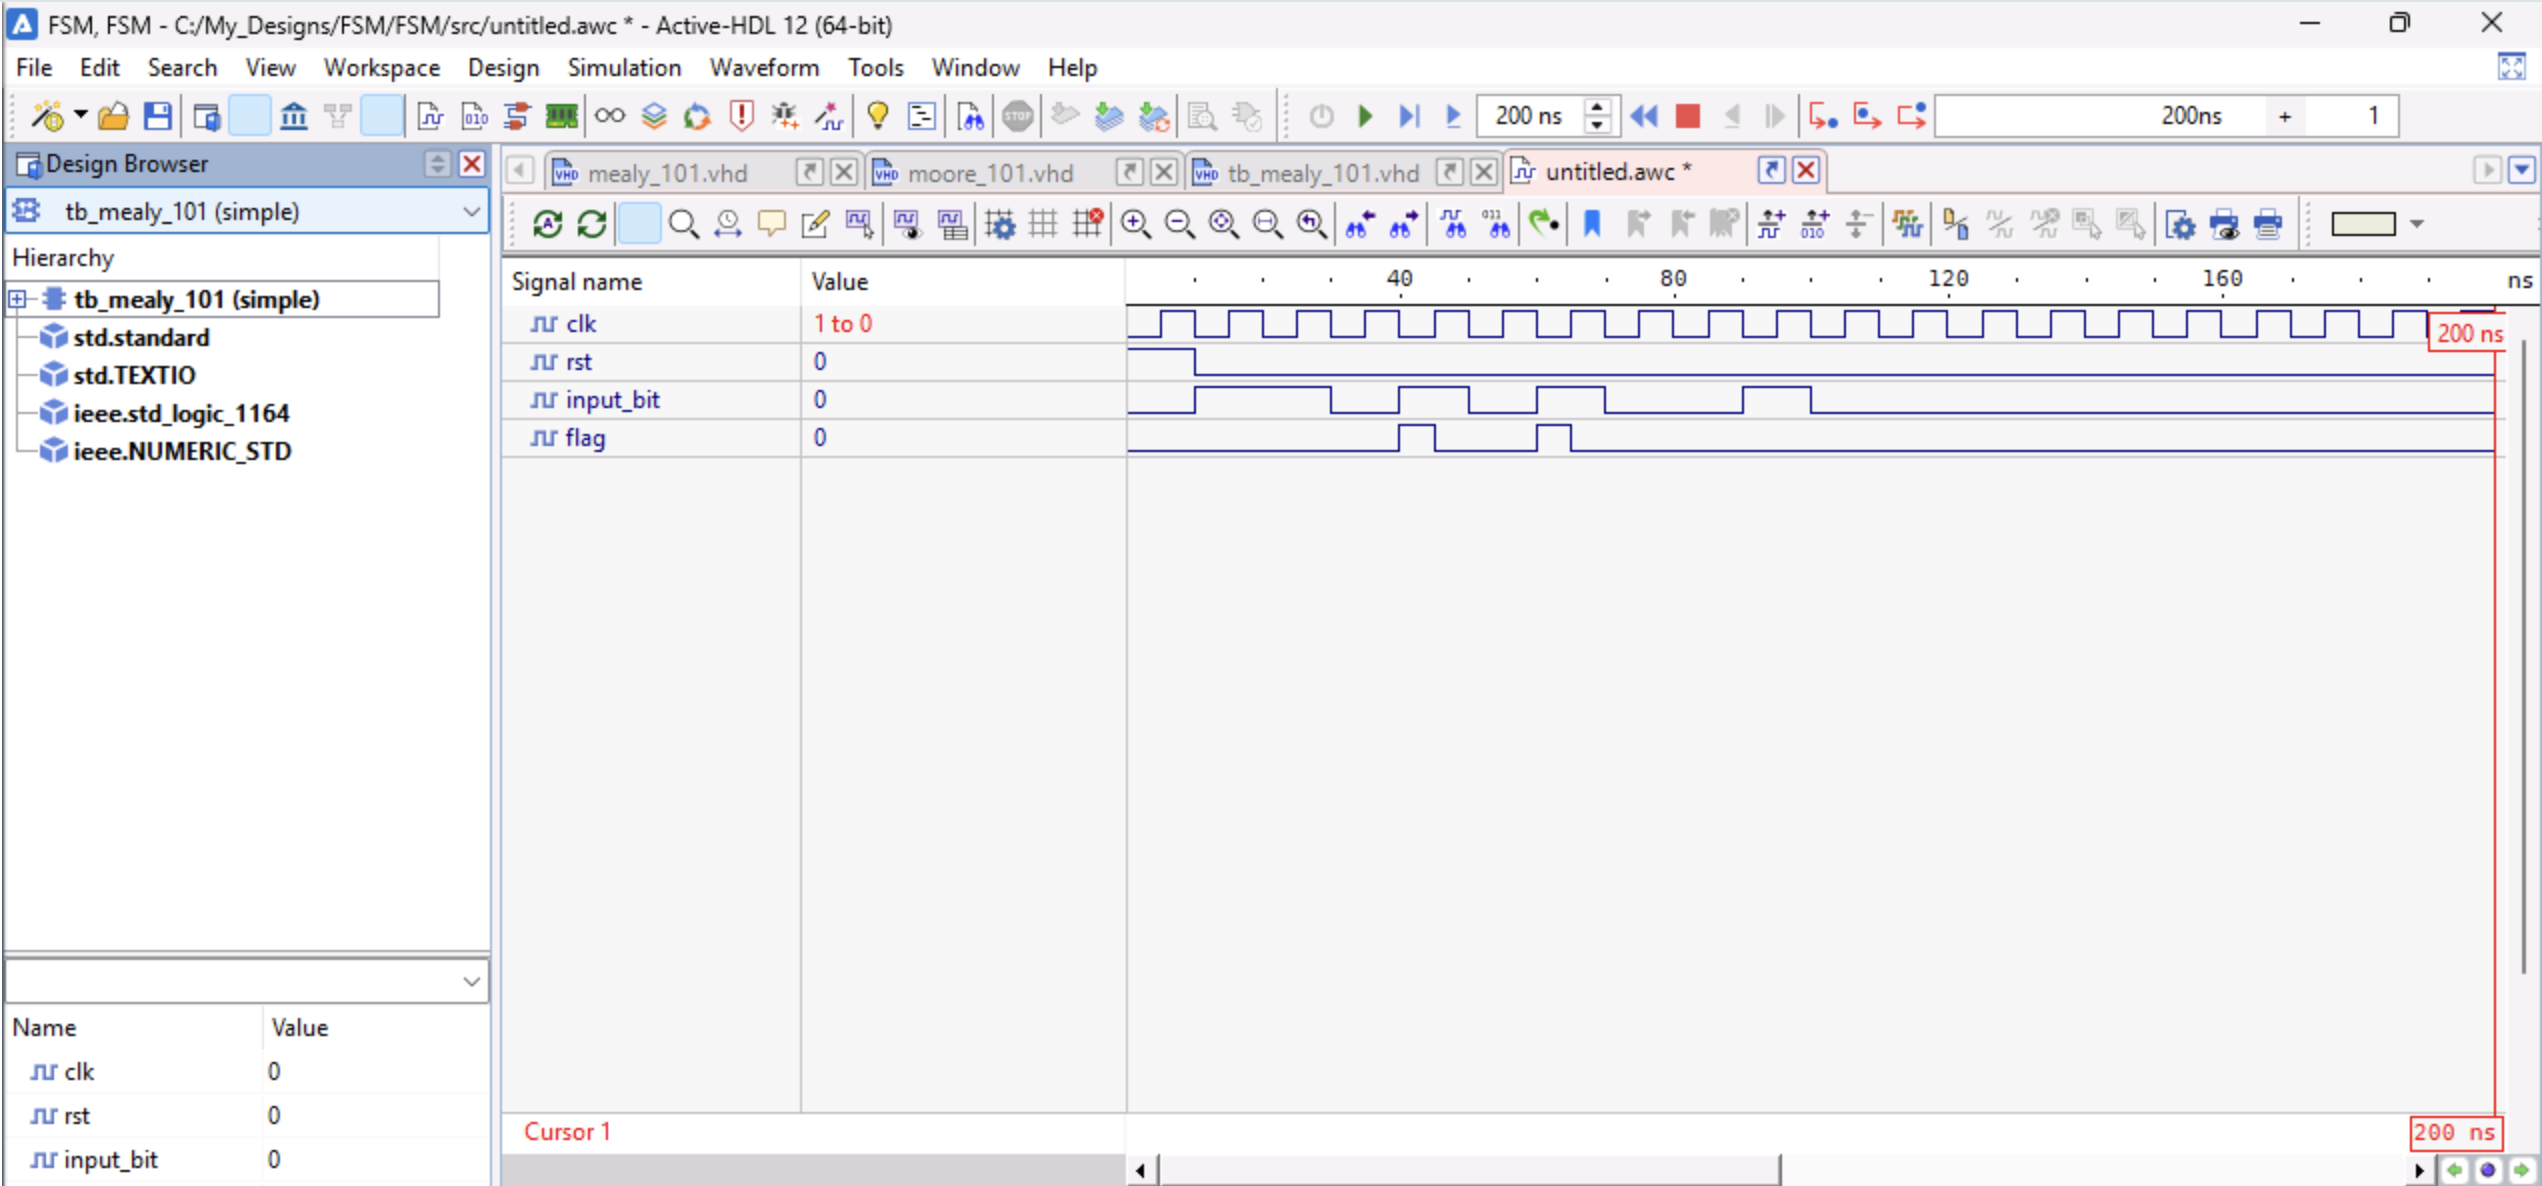
\includegraphics[width=\textwidth]{sim_mealy.png}
\caption{Simulación del detector Mealy: la salida \texttt{flag} se activa en el mismo ciclo en el que llega el último \texttt{1} de la secuencia.}
\label{fig:mealy}
\end{figure}

Este comportamiento confirma la propiedad fundamental del modelo Mealy: la salida es función combinacional de estado y entrada. Por ello \texttt{flag} sigue de cerca a \texttt{input\_bit} cuando la máquina está en S2, y vuelve a cero en cuanto la entrada cambia. La máquina no requiere un estado dedicado a la aceptación, lo cual reduce el conteo a tres estados.

\subsection{Detector Moore de la secuencia 101}
La Figura~\ref{fig:moore} muestra la simulación del detector Moore. La máquina recorre los mismos estados intermedios que la versión Mealy, pero la salida \texttt{flag} solo se activa cuando se entra al estado S3, es decir, en el ciclo posterior al último \texttt{1} de la secuencia. Esto se observa con claridad al alinear los pulsos de \texttt{flag} con \texttt{input\_bit}: cada activación aparece desplazada un período de reloj respecto al instante en el que se completó el patrón.

\begin{figure}[H]
\centering
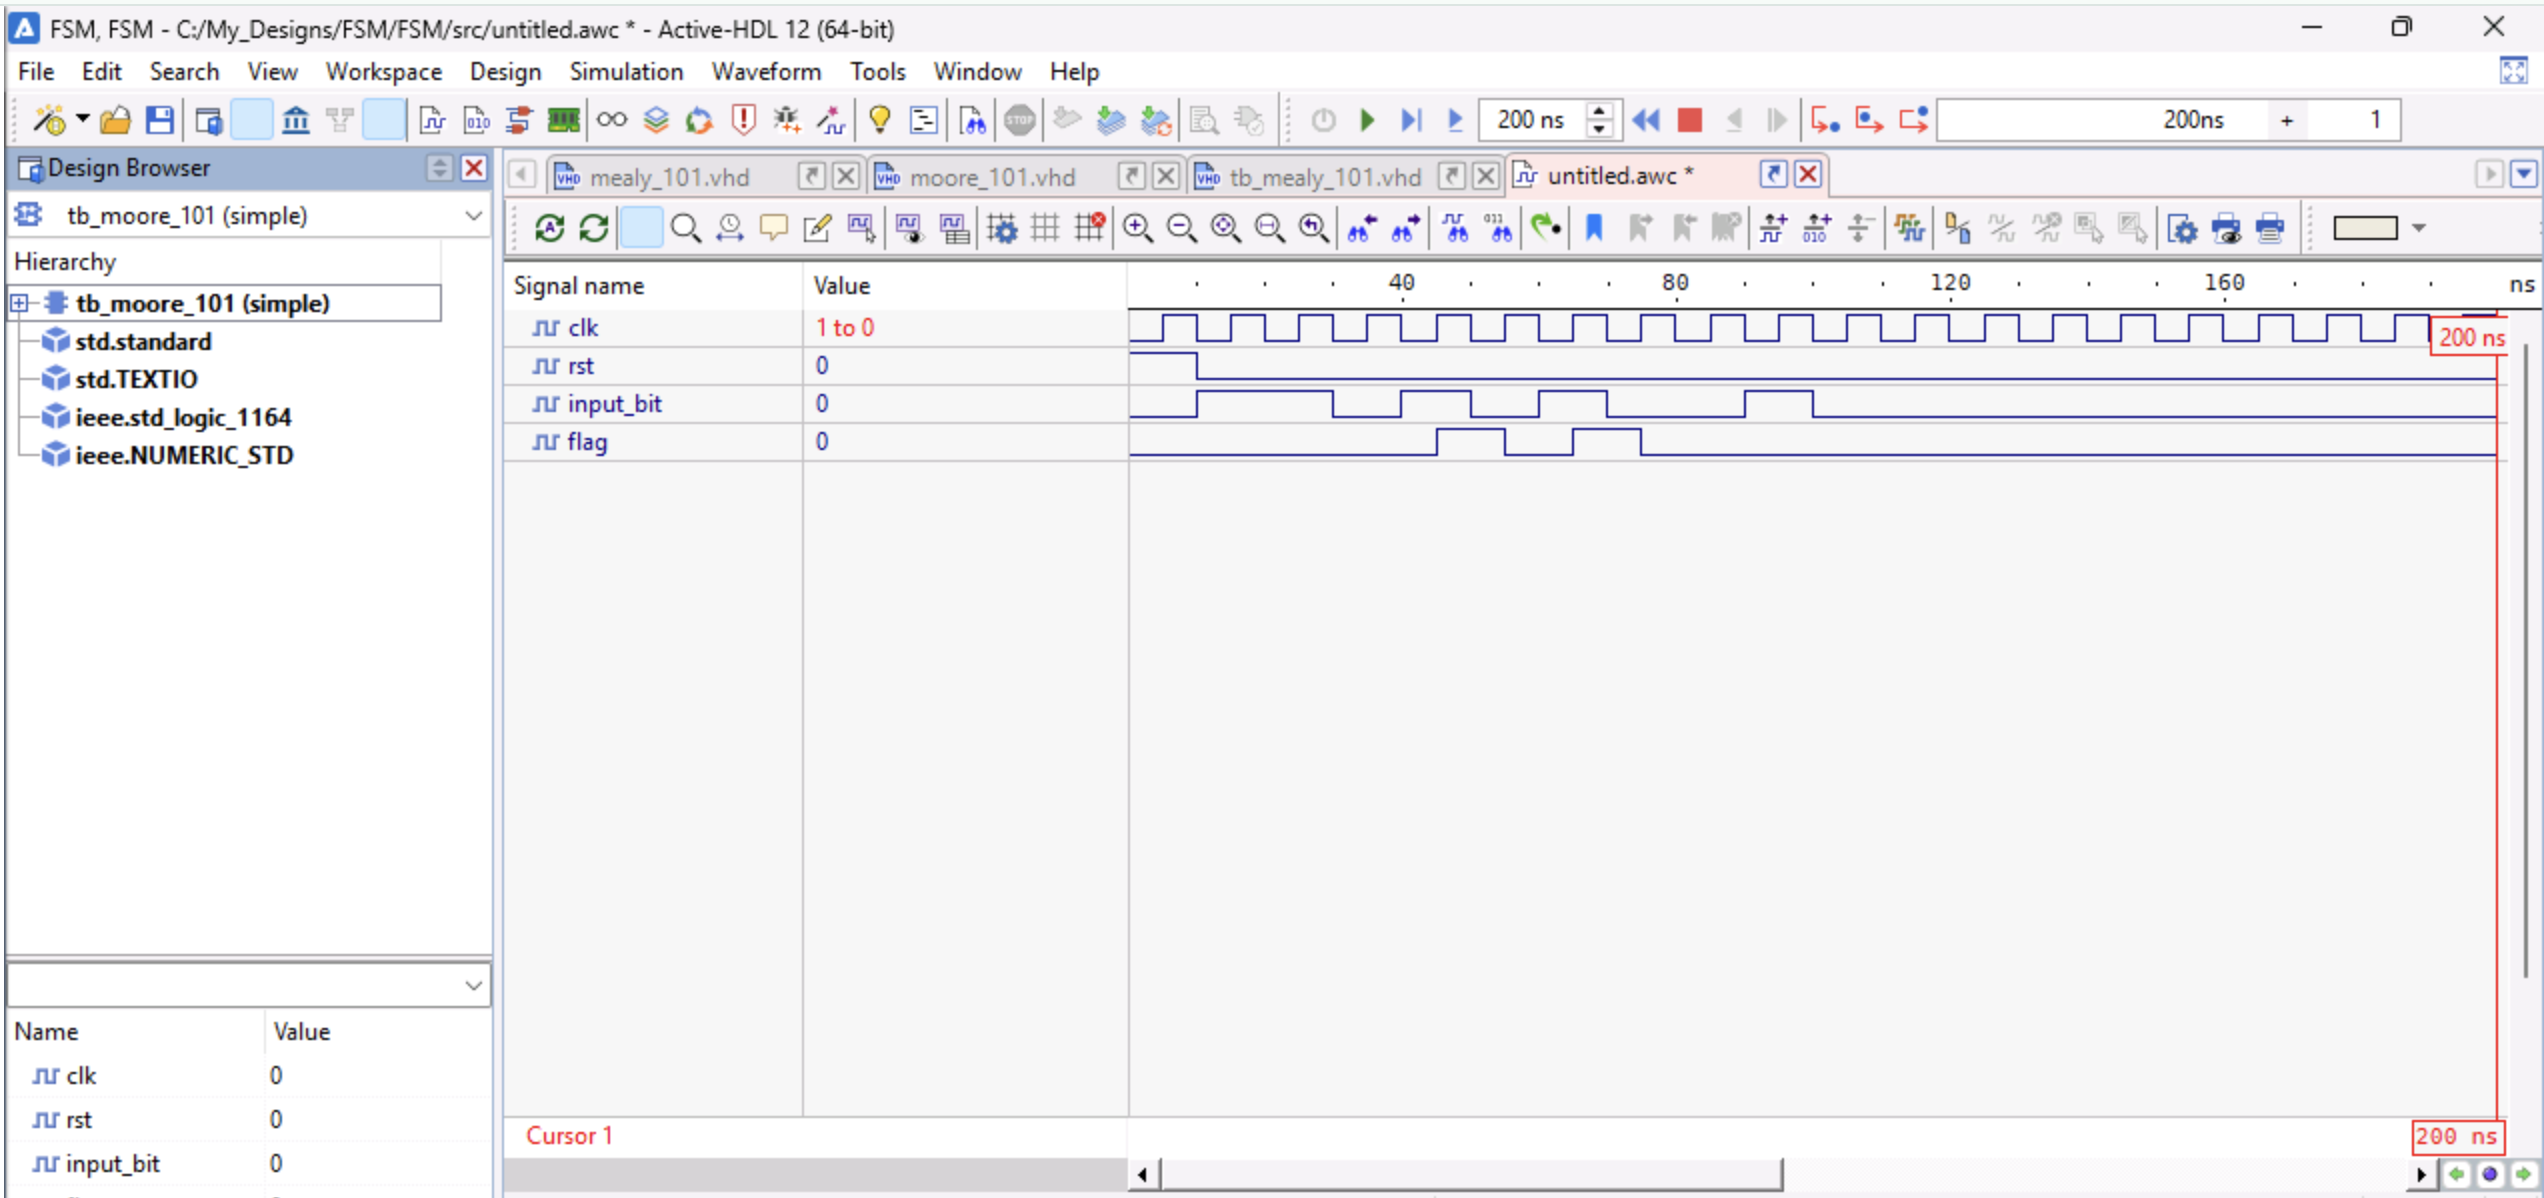
\includegraphics[width=\textwidth]{sim_moore.png}
\caption{Simulación del detector Moore: \texttt{flag} se activa al entrar al estado S3, un ciclo después del último bit de la secuencia.}
\label{fig:moore}
\end{figure}

La introducción del estado S3 hace que la salida quede registrada al estado y no presente transitorios derivados de la entrada, a costa de un retardo de un ciclo. Esta propiedad es precisamente la que se busca cuando la salida de la FSM se conecta a otro bloque registrado, ya que evita carreras críticas y facilita el cumplimiento de los tiempos de \textit{setup}.

\subsection{FSM del semáforo}
La Figura~\ref{fig:sem} muestra la simulación de la FSM del semáforo en aislamiento. Se observa el avance ordenado por los estados S0, S1, S2, S3, S4 y S5 (codificados respectivamente como \texttt{01}, \texttt{02}, \texttt{04}, \texttt{08}, \texttt{10} y \texttt{20} en hexadecimal por la codificación \textit{one-hot}) y el regreso cíclico a S0. La señal \texttt{counter} incrementa en cada flanco activo y dispara la transición cuando alcanza \texttt{timeout\_value}, que a su vez se ajusta al valor del estado en curso. Las salidas \texttt{luz1}, \texttt{luz2} y \texttt{luz3} cambian de acuerdo con la Tabla~\ref{tab:semaforo_estados}.

\begin{figure}[H]
\centering
\includegraphics[width=\textwidth]{sim_semaforo.png}
\caption{Simulación de la FSM del semáforo: secuencia cíclica de los seis estados y luces correspondientes a las dos vías y al cruce peatonal.}
\label{fig:sem}
\end{figure}

Si en la simulación se activara la entrada \texttt{emergency}, la FSM regresaría al estado S0 y la asignación de salidas dejaría \texttt{luz1=001}, \texttt{luz2=001} y \texttt{luz3=01}, condición segura en la que ambas vías quedan en rojo y el peatón en rojo. Esto valida el camino de control de emergencia y confirma que la FSM responde correctamente a una señal asíncrona de servicio.

\section{Análisis de resultados}

La comparación entre las dos arquitecturas del detector \texttt{101} confirma las diferencias teóricas estudiadas en el curso. La FSM Mealy resuelve la detección con tres estados y reacciona en el mismo ciclo en el que llega el último bit; la FSM Moore necesita cuatro estados pero produce una salida estable y registrada con un retardo de un ciclo. En sistemas pequeños como éste, ambas opciones son válidas, pero la elección depende del entorno: cuando la salida alimenta lógica combinacional sensible a transitorios, conviene Moore; cuando se requiere mínima latencia, conviene Mealy. La forma en que se permitieron las detecciones traslapadas (regresar a S1 desde S2 o S3 al recibir un \texttt{1}) es la misma en ambos casos y se comprueba en la simulación al observar dos activaciones consecutivas de \texttt{flag} sobre la subcadena \texttt{10101}.

En la FSM del semáforo, la relación entre \texttt{current\_state}, \texttt{next\_state} y \texttt{timeout\_value} muestra que la transición entre estados no ocurre de forma inmediata sino únicamente cuando el contador alcanza el tiempo asignado al estado actual. Este comportamiento confirma que la temporización fue integrada correctamente dentro de la máquina y que cada fase permanece activa durante el intervalo programado. En una implementación sobre la PYNQ~Z1 el contador se alimentaría desde un divisor de frecuencia de \SI{50}{\mega\hertz} a \SI{1}{\hertz}, integrado a la FSM mediante un módulo estructural superior; en simulación, los tiempos se interpretan directamente como ciclos del reloj de prueba.

Las salidas observadas para las luces vehiculares y peatonales coinciden con la asignación planeada en cada estado. La codificación \textit{one-hot} del estado facilitó la lectura del \textit{waveform} y, en una eventual síntesis, permitiría implementar el registro de estado con seis biestables individuales, lo cual suele ser eficiente en FPGA.

\section{Buenas prácticas}
Durante el desarrollo se mantuvieron las convenciones que ya se habían adoptado en prácticas anteriores: separación clara entre lógica secuencial y combinacional, asignaciones por defecto al inicio de los procesos combinacionales para evitar latches no deseados, uso exclusivo de \texttt{numeric\_std} para aritmética sobre vectores y descripción de los módulos con interfaces mínimas. La codificación \textit{one-hot} del estado en la FSM del semáforo se eligió por simplicidad de lectura en el \textit{waveform} y porque suele inferir registros eficientes en FPGA.

\section{Conclusiones}
Se diseñaron y verificaron en VHDL tres FSM con propósitos distintos: dos detectores de la secuencia \texttt{101} (uno Mealy y otro Moore) y una unidad de control para un semáforo de doble vía con cruce peatonal. La simulación en Active-HDL confirmó las diferencias de temporización entre los modelos Mealy y Moore: el primero activa la salida en el mismo ciclo en el que se completa la secuencia, mientras que el segundo lo hace un ciclo después al depender únicamente del estado. Ambas implementaciones permiten detecciones traslapadas y son consistentes con el comportamiento teórico esperado.

La FSM del semáforo recorrió correctamente los seis estados, respetó los tiempos asignados a cada fase mediante el contador interno y la señal \texttt{timeout\_value}, y dejó preparado el camino de control de emergencia. En una integración posterior sobre la PYNQ~Z1 esta FSM se uniría a un divisor de frecuencia de \SI{50}{\mega\hertz} a \SI{1}{\hertz} mediante un módulo estructural superior, permitiendo que los tiempos definidos en \texttt{timeout\_value} correspondan a segundos reales.

Esta práctica reforzó el manejo de procesos secuenciales y combinacionales en VHDL, así como la importancia de las FSM como base de las unidades de control en arquitecturas computacionales.

\section{Referencias}
\begin{thebibliography}{9}
\bibitem{manual_practica}
O. Guillén Fernández. \textit{Práctica 4: Máquinas de Estado Finito (Control Unit)}. Universidad de las Américas Puebla.

\bibitem{ashenden}
P. J. Ashenden. \textit{The Designer's Guide to VHDL}. Morgan Kaufmann, 2008.

\bibitem{harris}
D. M. Harris and S. L. Harris. \textit{Digital Design and Computer Architecture}. Morgan Kaufmann, 2nd ed., 2012.

\bibitem{ieee_vhdl}
IEEE. \textit{IEEE Standard VHDL Language Reference Manual}. IEEE Std 1076.

\bibitem{active_hdl}
Aldec. \textit{Active-HDL Documentation}. Disponible en: \url{https://www.aldec.com/en/products/fpga_simulation/active_hdl}

\bibitem{ug585}
Xilinx. \textit{UG585: Zynq-7000 SoC Technical Reference Manual}. Disponible en: \url{https://www.xilinx.com/support/documentation/user_guides/ug585-Zynq-7000-TRM.pdf}
\end{thebibliography}

\section*{Repositorio del proyecto}
\addcontentsline{toc}{section}{Repositorio del proyecto}

El código fuente VHDL de las tres FSM, junto con las capturas de las formas de onda obtenidas en Active-HDL, se encuentra disponible en el siguiente repositorio público de GitHub:
\begin{center}
\url{https://github.com/Robbienicur/Arquitecturas-Computacionales/tree/main/Practica-4}
\end{center}
La carpeta \texttt{Practica-4} del repositorio contiene los archivos \texttt{mealy\_101.vhd}, \texttt{moore\_101.vhd} y \texttt{fsm\_semaforo.vhd}, las imágenes de la simulación y este mismo reporte en formato PDF.

\end{document}
